\documentclass[10pt,a4paper,twocolumn,twoside]{article}
\usepackage[utf8]{inputenc}
\usepackage[catalan]{babel}
\usepackage{multicol}
\usepackage{graphicx}
\usepackage{fancyhdr}
\usepackage{times}
\usepackage{titlesec}
\usepackage{multirow}
\usepackage{lettrine}
\usepackage[top=2cm, bottom=1.5cm, left=2cm, right=2cm]{geometry}
\usepackage[figurename=Fig.,tablename=TABLE]{caption}

\usepackage[table,xcdraw]{xcolor}
\usepackage{tabularx}
\usepackage{float}

\usepackage{biblatex}
\addbibresource{ref.bib}

\captionsetup[table]{textfont=sc}

\author{\LARGE\sffamily Christian Espinosa Reboredo}
\title{\Huge{\sffamily Recognition of epileptic seizures from EEG data}}
\date{}

\newcommand\blfootnote[1]{%
  \begingroup
  \renewcommand\thefootnote{}\footnote{#1}%
  \addtocounter{footnote}{-1}%
  \endgroup
}

%
%\large\bfseries\sffamily
\titleformat{\section}
{\large\sffamily\scshape\bfseries}
{\textbf{\thesection}}{1em}{}

\begin{document}
\nocite{*}
\fancyhead[LO]{\scriptsize AUTOR: Christian Espinosa Reboredo}
\fancyhead[RO]{\thepage}
\fancyhead[LE]{\thepage}
\fancyhead[RE]{\scriptsize EE/UAB TFG INFORMÀTICA: Recognition of epileptic seizures from EEG data}

\fancyfoot[CO,CE]{}

\fancypagestyle{primerapagina}
{
   \fancyhf{}
   \fancyhead[L]{\scriptsize TFG EN ENGINYERIA INFORMÀTICA, ESCOLA D'ENGINYERIA (EE), UNIVERSITAT AUTÒNOMA DE BARCELONA (UAB)}
   \fancyfoot[C]{\scriptsize ``Mes'' de 20xx, Escola d'Enginyeria (UAB)}
}

%\lhead{\thepage}
%\chead{}
%\rhead{\tiny EE/UAB TFG INFORMÀTICA: TÍTOL (ABREUJAT SI ÉS MOLT LLARG)}
%\lhead{ EE/UAB \thepage}
%\lfoot{}
%\cfoot{\tiny{February 2015, Escola d'Enginyeria (UAB)}}
%\rfoot{}
\renewcommand{\headrulewidth}{0pt}
\renewcommand{\footrulewidth}{0pt}
\pagestyle{fancy}

%\thispagestyle{myheadings}
\twocolumn[\begin{@twocolumnfalse}

%\vspace*{-1cm}{\scriptsize TFG EN ENGINYERIA INFORMÀTICA, ESCOLA D'ENGINYERIA (EE), UNIVERSITAT AUTÒNOMA DE BARCELONA (UAB)}

\maketitle

\thispagestyle{primerapagina}
%\twocolumn[\begin{@twocolumnfalse}
%\maketitle
%\begin{abstract}
\begin{center}
\parbox{0.915\textwidth}
{\sffamily
%\textbf{Resum--}

%\end{abstract}
%\bigskip
%\begin{abstract}
%\bigskip
%\\
\textbf{Abstract--}An electroencephalogram (EEG) is a test that detects electrical activity of the brain. This paper tries to go a step further to interpret seizures from electroencephalograms using deep learning algorithms. The data used in this paper is a public dataset CHB-MIT\cite{goldberger2000physiobank} of recordings of paediatric subjects with intractable seizures. Different methods of data processing are done and documented to make the most of the algorithms used as well as the strategy. The objective is to train an algorithm to classify when the subject is having a seizure and when it’s not.
\\
\\
\textbf{Keywords-- }electroencephalogram, deep learning, brain activity, classification, EEG analysis\\
}

\bigskip

{\vrule depth 0pt height 0.5pt width 4cm\hspace{7.5pt}%
\raisebox{-3.5pt}{\fontfamily{pzd}\fontencoding{U}\fontseries{m}\fontshape{n}\fontsize{11}{12}\selectfont\char70}%
\hspace{7.5pt}\vrule depth 0pt height 0.5pt width 4cm\relax}

\end{center}

\bigskip
%\end{abstract}
\end{@twocolumnfalse}]

\blfootnote{$\bullet$ E-mail de contacte: 1459024@uab.cat}
\blfootnote{$\bullet$ Menció realitzada: Computació }
\blfootnote{$\bullet$ Treball tutoritzat per: Aura Hernández Sabaté (Ciencies de la Computació)}
\blfootnote{$\bullet$ Curs 2021/22}

\section{Introduction}
\leavevmode\\
\lettrine[lines=3]{A}{n} epileptic seizure is a period of symptoms due to abnormally excessive or synchronous neuronal activity in the brain. This can cause different effects like uncontrolled shaking movements involving much of the body, parts of the body or subtle momentary loss of awareness. In order to understand this issue, it is important to understand how neurons work and interact with each other to conserve what we call consciousness, represented as brain activity and brainwaves.
\\\\
Neural oscillations are rhythmic or repetitive patterns of neural activity in the central nervous system which can be driven by mechanisms within individual neurons or by interactions. Since 1824 neural oscillations have been observed, fifty years later intrinsic oscillatory behaviour was encountered in vertebrate neurons, but the purpose of these is yet to be fully understood.
\\\\
The main objective is to classify seizures from brain activity. First of all, it will be needed an inside view on how the brain works to have a hint on how and what is done to extract or intercept information from the neurons to process externally in a computer. This information is available annexed in this paper just to have an overview to further understand the subject. This matter is not the main purpose of this paper as it specifies in data processing, architecture, model strategies and classification results.
\\\\
In this TFG it’s detail the complete process of epileptic seizure detection, from data processing to seizure recognition. Because this TFG works as a pipeline of different stages, an insight view of each is done, starting from data processing from a well-known database (CHB-MIT) of encephalograms collected from 23 subject with interactable seizures that has been used in previous research. Followed by the strategy of the architecture used to classify the signals to finally understand the classified results into seizure and not seizure.
\\\\
There have been many other projects about seizure recognition, so in this project another approach is done to further study this subject. Before starting, an overview of different similar projects is done. Also, the scripts done in this TFG have been done with the help of the CVC team working on related projects.


\section{Related Work}
\label{sec-related-work}
A lot of research has been made of the brain to further understand it’s capabilities using deep learning algorithms. Below are different projects attempting to interpret and process EEG data in order to define a baseline of what has been done so far. 
\\
\subsection{Mental Workload Detection based on EEG Analysis}
\label{subsec-work1}
A study of mental workload is done in order to work more efficiently, healthier and to avoid accidents since workload compromises both performance and awareness. The use of EEG signals has a high correlation with specific cognitive and mental states such as workload, proposing a binary neural network to classify EEG features across different mental workloads.
\\
Mental workload is defined as “the cognitive and psychological effort to conclude a task”, observing that depending if workload is too heavy or too light this can affect human performance. Also, since workload involves neuro-physiologic, and perceptual processes it is affected by individual capabilities, motivation to preform, physical and emotional state which it’s multifaceted nature of workload prevents it of studying directly but it is feasible to infer this from a number of quantifiable variables.
\\
There are two main categories to measure workload:
\\
\begin{itemize}
\item Subjective measures: Being the most used to asses mental workload, the NASA Task Load Index (TLX) a prominent way to gain insight on perceived workload from the subject based on a weighted average of six sub-variables: mental demand, physical demand, temporal demand, performance, effort and frustration. Widely used in aviation to assess mental workload of the pilot but it is highly subjective.
\item Physiological measures: Providing a more reliable data by measuring physiological dynamic changes which cannot be controlled consciously, so that is why it’s more reliable. Readings such as electrocardiogram (ECG), electromyograph, electroencephalogram (EEG), photoplethysmography, respiration rate sensors, electro-dermal activity (EDA), oxygen density in the blood in the brain, and eye movement trackers... The combination of inputs reports better accuracy than the analysis if each one independently.
\end{itemize}
\leavevmode\\
The approach is to investigate the ability of 1D-CNN models to recognise two types of mental load from EEG signals and to generalise the model to a population not seen in the training set. They use N-back test (memory demanding games requiring the resolution of simple arithmetic operations adjusting workload) to induce low and medium workload and to classify a simple neural network (NN) it’s trained using only the power spectrum of theta waves. Proposing a personalized model for each individual and a generalist one, preform the models in a dataset of 16 subjects showing outstanding results in a leave-one-out subject test and so generalizing to new unseen subjects.
\\
The method to obtain data all 16 subjects had to first watch a 10-minute relaxing video and afterwards do the N-back-test low, medium and high difficulty. Finally subjects ask a TLX questionnaire for subjective perception of the test difficulty and workload.
\\
To get the data itself EEG recordings were done using EMOTIV EPOC+ headset which has 14 electrodes placed according to the 10/20 system which provide raw data and power spectrum for the main brain rhythms (theta, alpha, beta low, beta high, and), at 128 Hz and 8 Hz, respectively. Data had to be filtered from noise with Inter Quartile Range (IQR) strategy to detect outlier values associated to muscular movement wave peaks. In this work, power spectrum used was from theta wave (4-8Hz) sampled at 8Hz feed into the models in 5 second windows of every electrode (14 EEG sensors). Variables were normalized to have 0 mean and
sigma=1 using the mean and standard deviation of the training set. 
\\
Networks have a hidden layer of 128 neurons with ReLU as the activation function. Before the classification layer a dropout layer was added to avoid overfitting and all models have been trained using weighted cross-entropy loss, to compensate the different lengths of base line and workload phases which introduces unbalance in data samples.
\\
In conclusion its reported 95\% confidence interval for each class computed for all subjects and recall above 90\%. It is suggested to use longer windows to capture EEG non stationary nature.
\\
%\subsection{EEG SIGNAL DIMENSIONALITY REDUCTION AND CLASSIFICATION USING TENSOR DECOMPOSITION AND DEEP CONVOLUTIONAL NEURAL NETWORKS}
%\label{subsec-work2}
\section{Objectives}
\label{sec-objectives}
The main goal in this TFG is to detect seizures from the dataset CHB-MIT. To fulfil the objective an architecture has been created working within a pipeline of events. Starting by finding the best data analysis and processing method before feeding it to the deep learning algorithms. There are many sub-objectives to be completed to obtain good results from this architecture and also, it’s modular for further expansion and studies. The main strategy of the scripts execute in sequence:
\\
\begin{figure}[h!]
    \caption{Scheme of data processing }
    \centering
    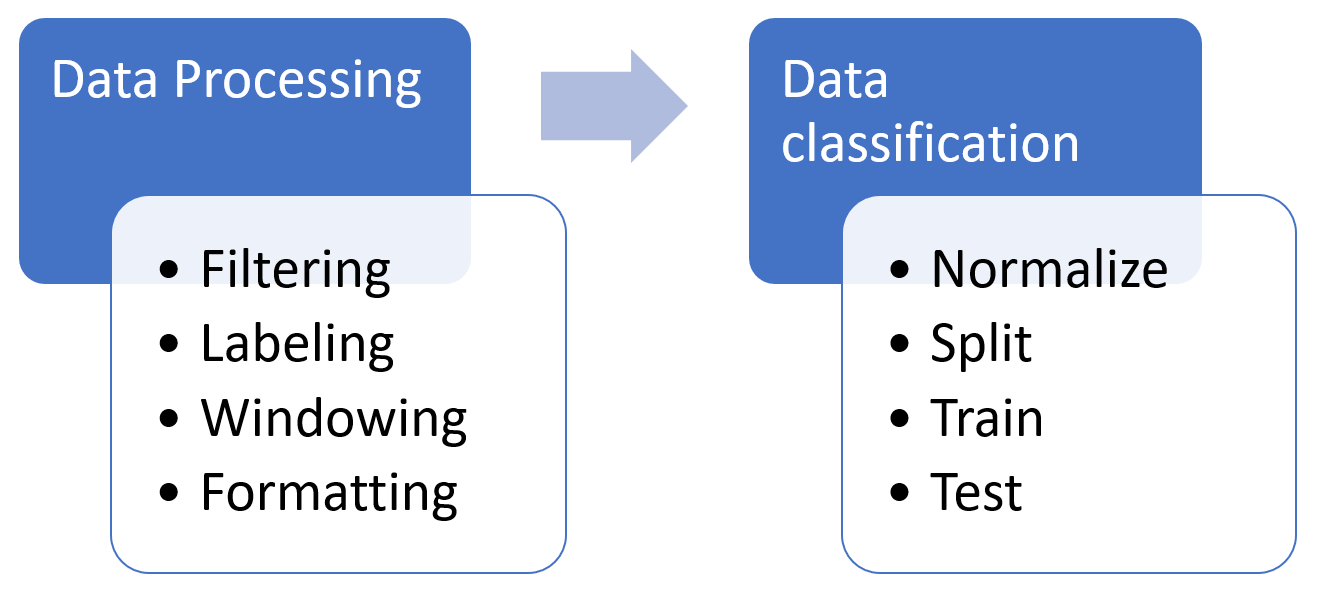
\includegraphics[width=0.5\textwidth]{img/pipeline.png}
\end{figure}
\\
To fulfil the objectives is crucial to define smaller objectives to make work easier. Within the first objective there are several important parts: 
\\
\begin{itemize}

    \item Raw data must be readable, as the data base CHB-MIT\cite{goldberger2000physiobank} is in European Data Format (EDF), a standard file format designed for exchange and storage of medical time series, so all files in the dataset are “.edf”. A script has been programmed to save .edf files into .parquet format.
    \item Setting different functions to filter data making sure data fits certain constraints to obtain better results when training the model.
    \item Get the labelling data, to have a ground truth from the recorded data. This part is essential to understand if the model works as expected.
    \item Define different functions to define how data enters the model to be trained. There are many ways information can be extracted from data. 
    \item Each model needs to be configured to accept the dimensionality of the data fed to it.
    \item Work different models to choose what models give better answers form input data.
    \item After all the models results, an overview is done to understand the results and conclude the best way to treat this database, for further investigation.

\end{itemize}
\section{Methods}
\subsection{Dataset}
The dataset is data collected from the Children’s Hospital Boston, consisting in EEG recordings of subjects with intractable seizures. The folders classify in 23 cases from 22 subjects (case chb21 and chb1 are the same but 1.5 years apart). The subject’s personal information gender and age is in a separate file called SUBJECT-INFO added in this paper as subject\_info.csv.
\\\\
Each case contains between 9 and 42 edf files. There are edf files of EEG signals without seizures and others with recordings of seizures, these defined in RECORDS-WITH-SEIZURES. The files with seizures have the extension edf.seizures which disables the possibility of accessing the file with a normal edf reader library.
\\\\
Most cases have 1 hour of EEG recordings, but some have 1 to 4 hours depending on the case, split between 9 to 42 edf recordings, recorded at 256Hz in 16 bit resolution. It’s important to note, some subjects had hardware interruptions while the recording of the EEG, and so when there is an interruption, it’s noted in the summary.txt file. This kind of interruptions are a problem to get information normally, because the disposition of the electrodes change making it harder to control the disposition of the electrodes and the EEG might not work for a sequential approach, for example, if it’s important there is hypothetically an order on how a seizure comes to be, this file would certainly be discarded. To take into account this file the script to process the data in this TFG should be programmed to do so. For now, the objective is different, this project just classifies if there is or not a seizure, but for further development it should be considered. The data base is very large containing enough uninterrupted data to work with.
\\\\
The data used to train the model in this TFG is data from subject 1 to subject 10. Also only few .edf in each subject’s folders have any seizure. If every .edf was used, there would be a lot of data labelled as not seizure than seizure data, so from each subject only the files with seizure are used. Even so, handling only files with seizures the dataset is unbalanced, so for future development two strategies should be considered:

\begin{itemize}
  \item Files should be cut to have a balance of labelled data of 50\% data with seizure and 50\% data without. This strategy could end up un subsampling, considering there are few seizures in the hole dataset.
  \item When training the model, the criteria of cross Entropy should be weighted. To consider no seizure less important than seizure data.
\end{itemize}
\leavevmode\\
\subsection{Data processing}
Because in this TFG the CHB-MIT Scalp EEG Database is being used and all files are in format edf, a first script has been needed to process data, called “03\_ReadEDF.py”.
\\\\
In the “03\_ReadEDF.py” script there are different options on how raw data is imported, and also there are options on the way to execute them. During the development of this TFG many tests have been done, there for there are two different ways to execute the script:
\\
\begin{itemize}
  \item Single execution, where the subject number and the edf file of the subject needs to be provided to execute the script for this single file. 
  \item Multiple executions, where the number of subjects is provided. The script will go through all the first n subjects defined.
\end{itemize}
\leavevmode\\
It’s designed to extract the files from a specific folder hierarchy where all the encephalograms are classified by subjects. For simplicity this script obtains, filters, plots, and saves in parquets all input data. Afterword’s it also labels the data and splits it into windows so the model can process data easily. 
\\\\
The script will automatically label all raw data using the summary file in each subject’s folder, so it’s important for it to be present or a label execution error will pop up. The files edf.seizures in every subject’s folder were unreadable, even reading the binary was a failure. The script will make sure the file has all the data from the desired electrodes, this is important because there were hardware problems while recording the edfs, some files have gaps or lack some data, if any edf file has this problem it will automatically be excluded and the user will be notified. Each one has 22 different channels, which are the electrodes of the subject. In order to label the data, a new column is created (the 23rd) as seizure with the information of every row being a seizure or not and also a 24th column to set the observation windows for the model.
\\\\
Filtering data is done by first setting a maximum range from 0.5hz to 50hz, and afterwards only by changing the name of a parameter it can be changed to delta, theta, alpha, beta or gamma’s range frequencies in a dictionary added by default. Everything is modular so it can be changed any time with any range of frequencies. All data is saved in parquet format in a different folder, if plotting is enabled it will plot each subject’s data.
\\\\
Once the data is filtered and labelled it`s saved two numpys, one “file\_data\_x.npy” and “file\_data\_y.npy”. In data\_x the file has a numpy array of three dimensions containing number of windows, electrodes and values. In data\_y there are two dimensions, number of windows and window\_seizure which defines if the window has a seizure in it with a 1 or not with a 0. 
\\\\
With this, all the parquets and arrays are specifically saved and ordered to ensure easy access and fast comprehension of the hierarchy of folders. The database folder has every subject in a separate folder and inside individual folders for edf, parquets, numpys and results.
\\
\begin{figure}[h!]
    \caption{Filtered data in Theta range from electrode FP1-F7, subject 1 file 3}
    \centering
    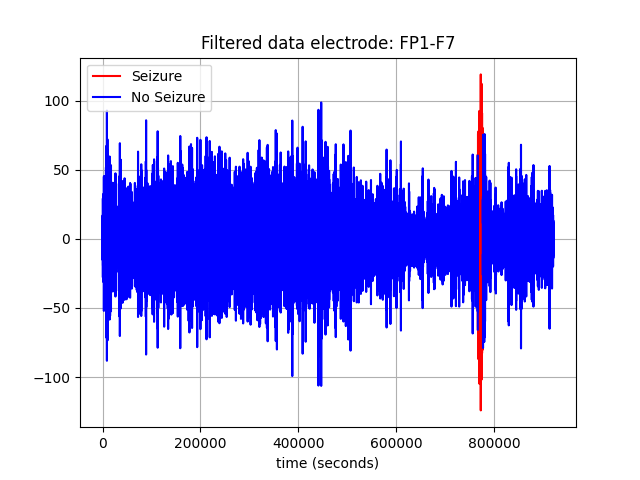
\includegraphics[width=0.5\textwidth]{img/seizurenoseizure.png}
\end{figure}

\leavevmode\\
\subsection{Network}
An already done deep learning algorithm is used from the research group IAM from the CVC, which is working on a framework to determine the optimal architecture for cognitive state recognition from EEG signals, with the objective to answer different questions:
\\
\begin{itemize}
  \item How to combine the signals to create the input features for feature extraction? In this case, having 14 sensors x 5 wavelengths, so 70 raw signals. These signals can be concatenated, or projected.
  \item Which neural network is the best performer?
  \item Is it better to ensemble the different classifiers before combining the signals?
\end{itemize}
\leavevmode\\
This model was originally intended to study brain workload, so, with the help of this model it’s changed to fulfil the objective of clinic seizure detection. In this TFG, different strategies are applied on the input data of the algorithm to further study it’s capabilities as well as using different models to compare results between them.
\\\\
Once all desired raw data is filtered and saved, the second script to execute is “04\_MExecution.py”, this one is in charge of the execution of the model, training and testing to obtain the results classifying the data. All hyperparameters are defined at the beginning of the script as well as the declaration and initialization of the model. There are different typs of execution for development that can be enabled by boolean variables commented in the script. 
\\
\begin{itemize}
  \item CheckModel is the first way to execute the model, this one is needed to make sure the model works as intended before using real data to train it. It uses the selected model and feeds to it random data using torch with the defined parameters in the function.
  \item If the model works with no isues with CheckModel, then the training execution can begin. This first phase selects every numpy from n subjects defined at the beginning and trains the model with all the data. Every time the model finishes the epochs of a file, it saves the model in the database.
  \item In the second phase the previous trained model is loaded to test it and data is defined to set the normalization scalers for testing. For further development this should be changed to make an average of scalers by all trained data for example, or normalize data before the script’s execution. Once the model is tested a classification report is done using sklearn library and saved to a results folder in the subject’s folder.
\end{itemize}
\leavevmode\\
\\
The script uses numpy arrays as input data stored as previously mentioned in data\_x and data\_y. These files depending on the strategy of the script can be processed one last time to ensure good results from the classification. In this TFG data when loaded uses the strategy stated previously as phase 1 and 2, for training and testing. But the script has the option to split the files in train and test by a percentage variable. For the executions done this variable is set to 1 (100\%) on training, and 0 on testing phase.
\\\\
During the implementation of this script, a lot of problems of dependency on critical libraries has happened. Starting by cuda, for faster results it is used in all models, but it might not work if the architecture of the graphics card is too old. It is also not compatible with python 3.10 which was the version being worked on at the moment, it had to be switched to an environment with python 3.8 to avoid further issues. The script will be executed with cuda if the libraries are available, if not it will automatically work with the CPU.
\\\\
When it’s time to save the model, it’s saved in a folder called “trys” in the root directory, like if it was another subject but it only contains pt files, ordered in it by the date of execution.
\\\\
The models used in the TFG have similar structures. The first one CNN\_ConcatInput and the second one CNN\_ProjOut\_Conv. As the names suggest these models are Convolutional Neural Networks. Both models have 3 base layers of convolution defined by a function ConVNet which defines 3 different layers using torch, the first one being 16@22x19. The first parameter as number of input features defined by a constant variable defined in the constructor of the model, the second parameter defines the size of the data, 22 being the channels, in this case 
\\
\leavevmode\\
\begin{figure}[h!]
  \caption{Scheme of data dimension transformation through model CNN\_ConcatInput}
  \centering
  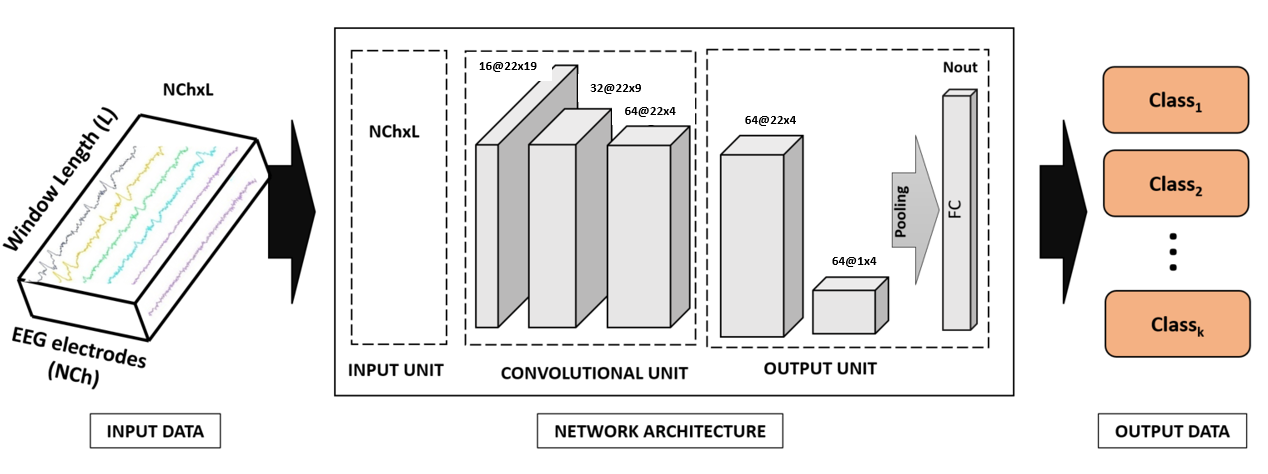
\includegraphics[width=0.5\textwidth]{img/FeatureProjectorModel CHM.png}
\end{figure}
\leavevmode\\
During the implementation of this procedure, a lot of problems of dependency on critical libraries has happened. Starting by cuda, for faster results it is used in all models, but it might not work if the architecture of the graphics card is too old. It is also not compatible with python 3.10 which was the version being worked on at the moment, it had to be switched to an environment with python 3.8 to avoid further issues.
\\


\section{Execution}
\leavevmode\\
The execution of the model has been made with all the previous procedures regarding data processing in this paper. Data from subject 1 to 10 has been used to train the model and data from 11 to 16 has been used to test the accuracy of the predictions of the model. For every file 50 epochs have been done to ensure a good understanding from the model of the data and a (3,1) kernel size.
\\\\
At first the strategy of training and testing the model was done within the files of the subjects. For each file it was split in two by a percentage variable and afterword’s it was trained and tested. This strategy was abandoned because it wasn’t as efficient as if many files where trained. Because there are few seizures in the hole database it makes it difficult to train a model to understand the existence of a seizure. Also, it was dependent on the position of data in the file, considering there are few or in most cases only one seizure, if the file was split one half would have a seizure and the other would not have one. This is a big problem if training has no seizure and the testing data has it, it will never be able to learn what a seizure is, and if its opposite, it might learn what a seizure is but it would never be possible to test if it learned correctly to classify.
\\\\
In the end the strategy of first training the model with some files and then with others do the testing, was the best way to go considering training each file took around 10 min depending on the computer it was executed with. There was a big difference between executing the model with and without cuda, the first model was executed without cuda because of the hardware architecture and it spent around 30 hours training the model, and with cuda half the time.
\\\\
It’s important to note using a desktop computer to train the model, considering it will get hot finishing the last epochs of every file. It’s also very resource consuming, considering it loads all the file to the RAM and reads and works with it from there. It could be a problem to many computers, some with 8Gb won’t work, only with 16Gb of memory worked for me. In most cases, the .edf files contain exactly one hour of digitized EEG signals, although those belonging to case chb10 are two hours long, and those belonging to cases chb04, chb06, chb07, chb09, and chb23 are four hours long; occasionally, files in which seizures are recorded are shorter, so the idea of concatenating files of a subject to have one file per subject it’s also excluded. 
\\


\section{Conclusion}
\subsection{Results}
\leavevmode\\
After training the two models with files from subjects 1 to 10, testing only took 15 to 30min to execute with subjects from 11 to 16. The results given by the function classification\_report of the library metrics from sklearn were saved in parquets and then loaded with “05\_ReadParquet.py” script, which reads every parquet from the folder results of every tested subject. 
\\\\
At first results looked promising viewing a staggering 95\% to 100\% accuracy in classification from the model. But upon further inspection the results are bad, because I realized the accuracy given by the report was because it predicted all data to be “no seizure”. So, the other 5% it’s the Seizure in the data that the model is classifying it as no-seizure. Because data is mainly one-sided to no-seizure the result 95% is because it was only classifying this class, so in the end it’s returning the percentage of the  amount of data of each class.
\\\\
Looking up the results and the model I realized the data in the input of the model is not exactly as expected. There are inconsistencies in the results, for example as shown in the next two tables the two tables should have the same dimensions but here it’s not the case:
\\

\begin{table}[]
    \caption{Results from subject chb14 file 6}
    \begin{tabularx}{\columnwidth}{ @{\extracolsep{\fill}} |c|c|c|c|}
        \hline
                        & \textbf{0} & \textbf{1}                 & \textbf{accuracy} \\ \hline
        \textbf{precision} & 0.983      & {\color[HTML]{FE0000} 0.0} & 0.983             \\ \hline
        \textbf{recall}    & 1.000      & {\color[HTML]{FE0000} 0.0} & 0.994             \\ \hline
        \textbf{f1-score}  & 0.997      & {\color[HTML]{FE0000} 0.0} & 0.994             \\ \hline
        \textbf{support}   & 358.00     & 2.0                        & 0.994             \\ \hline
    \end{tabularx}
\end{table}

\begin{table}[]
    \centering
    \caption{Results from subject chb14 file 11}
    \begin{tabular}{|l|l|l|}
        \hline
                        & \textbf{0} & \textbf{accuracy} \\ \hline
        \textbf{precision} & 1.0        & 1.0               \\ \hline
        \textbf{f1-score}  & 1.0        & 1.0               \\ \hline
        \textbf{support}   & 360.0      & 1.0               \\ \hline
    \end{tabular}
\end{table}


\subsection{Future Work}
\leavevmode\\
For future work it would be strictly necessary first of all, to change the chunker function defining the windows of all the files. So assuming the model works as it should, getting the right processed data would be enough to have a consistent result. If the result of the classification is not good enough, I would consider adding a weighted cross entropy loss to avoid so much one sided data, for the model to learn more uniformly.
\\\\
With better results the code could give more accurate results so the difference between models could be further proven, to understand the best strategy to obtain process data. Not only two models but all the models offered by the CVC (CNN\_ConcatInput, CNN\_ProjOut\_Conv, CNN\_ProjOut\_Concat, CNN\_ProjOut\_AvgW, CNN\_ProjChannel, CNN\_ProjChannel\_v2, Seq\_C1D, Seq\_C1D\_Ensemble).
\\\\
Regarding biological characteristics, other models that consider data sequences could be also utilised such as dominant sequence transduction models, like states Attention is All you Need paper to create a model and maybe consider classifying data in three classes, seizure, no seizure and pre-seizure. This would enable people to predict seizures and further understand the reason of them if these are linked to a sequence or pattern.
\\\\
Data processing with other ranges of frequencies would be another issue of research as well, because in this paper only theta frequencies are considered and all other excluded, but there’s also delta, alpha, beta, gamma to research with, and it would be interesting to find out if a model could learn better from other bandwidths, and classify which one’s are better for classifying seizures.
\\\\
The position of the electrodes has been taken care of in the processing script, in a way where if there is an interruption and electrodes are changed, then the file was automatically excluded. But this could be changed to match the data of the previous positions of the electrodes and the positions of the one’s after the interruption. This way more data could be used to train the models as well as maybe considering different Brodmann’s areas (explained in the annex), to give more importance to data coming from certain areas in the brain which could cause or give more information about the reason, detonation or existence of seizures.
\\\\
As this paper the model was trained with different subjects because there’s not enough data to train with, it should be considered if different people have the same “type of seizure” affecting in the learning of the model. If enough data from only one subject was enough to train the model, it should be considered if this model could also predict seizures in other subjects with the same problem. The seizure itself might change between subjects, so maybe it’s alright to train the model for now with different subjects to consider many possibilities. 
\\\\
Finally other datasets should be researched as well to have a big overview of the difference in data between datasets regarding the seizure issue. It’s hard to come by with any, but it could help a lot in the learning of models to find out how seizures come to be. Also, other scripts should be created to process data for the model to input the same way, with the same characteristics, as it’s done with this dataset. For sure, this would be much more time consuming.
\\

\section{Acknowledgments}
\leavevmode\\
In the production of this TFG there has been a lot of people involved helping me to make this project as it is right now. When I first started working with it Aura Hernandez and Debora Gil provided me with the code of the models to change and adapt to the dataset I have been working with in this TFG. Because this team is working on the Mental Workload Detection the they provided me with al sorts of scripts in models and data processing. I was able to make an idea of what I wanted, but because of the big difference on de datasets, the data processing scripts had to be redone completely.
\\\\
Once I was working with this TFG, mid-way I started to have problems in my lack of knowledge on how torch works and I desperately needed an in-depth insight on how the models were created and the reason of the internal structure. With Elias we have been doing all kind of reunions to further understand these issues and also considering other strategies on how to process data more efficiently.
\\\\
I would like to consider the effectiveness in response from Jordi Pons when there’s a problem or simply any doubt. It’s someone to surely rely one, he’s always around and willing to help, this attitude is well known and appreciated by all.
\\\\
Last but not list special thanks to my teacher Aura Hernandez helping me review, schedule and manage this project as important as it is. Much appreciated everyone who has showed interest in this project. I wouldn’t have done it, with any doubt, without the help of people so professional I have been working with, thank you all.
\\


\section{Bibliography}
\label{sec-bibliography}

\printbibliography

\section{Annex}
\label{sec-annex}

\subsection{Neuron and neural activity}
\label{subsec-neuron}

To further understand how brain activity works we first need to study a single neuron and its purpose. A neuron is an electrically excitable cell that has the function to communicate with other cells. It does it by nearly touching other cells called synapsis, transmits the message through its axon and delivers the message by synapsis to another cell. Neurons are typically classified into types based on their function:
\\
\begin{itemize}
  \item Sensory neurons: Which respond to stimuli of the sensory organs and send the signals to the spinal cord or brain.
  \item Motor neurons: Its axons originate in the brain and spinal cord and innervate the muscles to produce muscle movements.
  \item Projection fiber: Are neurons found in the central nervous system and only establish synapses with other neurons, these consist of efferent and afferent fibers uniting the cortex with the lower parts of the brain and with the spinal cord.
  \item Interneuron: Is a neuron of the central nervous system, usually small and with a short axon, that interconnects with other neurons, but never with sensory receptors or muscle fibres, allowing it to perform more complex functions.
\end{itemize}
\leavevmode\\
Neurons transmit electrical waves originating from a transient change of permeability in the plasma membrane. Their propagation is due to the existence of a potential difference that arises due to different concentrations of ions on either side of the membrane, as described by the Nernst potential, between the inner and outer part of the cell (typically -70 mV). For the transmission of nervous impulses to other neurons, these do it by synapse, being a structure to pass electrical or chemical signals to another neuron or effector cell, there are two types of synapses:
\\
\begin{itemize}
  \item	Chemical synapse: Electrical activity in the presynaptic neuron is converted into the release of a neurotransmitter that binds to the receptors located in the plasma membrane of the postsynaptic cell.
  \item	Electrical synapse: Is one in which transmission between the first neuron and the second is not by the secretion of a neurotransmitter, but by the passage of ions from one cell to another through gap junctions, small channels formed by the coupling of protein complexes, based on connexins, in closely adherent cells.
\end{itemize}

\leavevmode\\
These electrochemical processes when large numbers of neurons show synchronized activity, electric fields that they generate can be large enough to be detected outside the skull, and so using electroencephalography (EEG) or magnetoencephalography (MEG) brain activity can be recorded.
\\

\subsection{Structure}
\label{subsec-structure}
\leavevmode\\
Now that we know where brain activity originates from, we can further study how the brain structures. There are many parts in the brain, but for now we are going to focus on the cerebrum because it initiates and coordinates movement, regulates temperatures, speech, judgement, reasoning, problem-solving, emotions, learning…
\\
The cerebrum, it’s the largest part of the brain, it’s divided by the medial longitudinal fissure in two hemispheres, each of these hemispheres has an outer layer of grey matter, the cerebral cortex and an inner layer of white matter. The fact that these are separated gives the opportunity for lateralisation of brain functions, which is the tendency of neurological functions to specialise in one hemisphere or the other, but even though the cerebrum is separated, these are connected by the corpus callosum.
\\
The cortex is mapped into fifty different functional areas known as Brodmann’s areas, defined by its cytoarchitecture (cellular composition), or histological structure and organization of cells. One scheme widely used (from Korbinian Brodmann) splits the cortex into 52 different numbered areas of different cellular structure and different functions.
\\
Having clarified this brain structure, obtaining data with electrodes from brain activity, positioning of these is something to keep in touch with depending on what it’s being studied. The same goes for defining the dataset train and test data, to feed as input to the deep learning algorithm, opening a new field on how to treat and subdivide data to make the most of it.
\\

%\section*{Agraïments}


\end{document}

